\section{Thiết kế mô hình miền nghiệp vụ}\label{sec:domain-model}
\subsection{Luồng nghiệp vụ chính}\label{sec:business-flows}

\textbf{Luồng ra/vào qua cổng:}
\begin{itemize}
    \item Nhân viên mở mã QR cá nhân trên TMC Employee Portal và xuất trình tại máy quét của trạm cổng. Mã QR là mã động có chữ ký số và thời hạn hiệu lực ngắn (FR-02, NFR-SEC-05).
    \item Hệ thống xác thực mã QR: kiểm tra chữ ký và thời hạn của mã, trạng thái của QR credential, trạng thái hoạt động của nhân viên, trạng thái của trạm cổng và quy tắc chống quẹt lặp chiều (FR-11).
    \item Nếu mã QR không hợp lệ, hệ thống ghi nhận lần quét bị từ chối kèm lý do, hiển thị kết quả từ chối trên kiosk và không tạo giao dịch chấm công (FR-14, FR-15).
    \item Nếu mã QR hợp lệ, hệ thống ghi nhận lần quét được chấp nhận và gửi lệnh mở cổng xoay thông qua API của hệ thống cổng xoay hiện hữu (FR-12).
    \item Chỉ khi hệ thống cổng xoay xác nhận đã mở cổng, hệ thống mới ghi nhận giao dịch chấm công gồm nhân viên, thời điểm, trạm cổng và hướng vào/ra (FR-13), sau đó kiosk hiển thị kết quả chấp nhận. Thời gian từ lúc quét đến khi hiển thị kết quả không vượt quá 2 giây (NFR-PER-01).
    \item Nếu hệ thống cổng xoay không phản hồi hoặc báo lỗi, kiosk không thông báo mở cổng thành công (NFR-AVL-03); lần quét được ghi nhận là mở cổng thất bại để bảo vệ xử lý và để đối soát khi cần.
\end{itemize}

\textbf{Luồng đồng bộ dữ liệu nhân viên:}
\begin{itemize}
    \item Hệ thống định kỳ tiếp nhận thông tin nhân viên (mã nhân viên, họ tên, nhà máy, bộ phận, trạng thái làm việc) từ hệ thống HR/Payroll, là nguồn dữ liệu nhân sự chính thức (FR-01).
    \item Nhân viên mới đủ điều kiện được cấp QR credential (FR-02). Khi nhân viên bị vô hiệu hóa, QR credential đang hiệu lực của nhân viên đó bị thu hồi và thay đổi được phản ánh tại các trạm cổng (NFR-SEC-06).
\end{itemize}

\textbf{Luồng điều chỉnh, chốt kỳ và truyền dữ liệu:}
\begin{itemize}
    \item Khi phát hiện dữ liệu chấm công bị thiếu hoặc sai, nhân sự có thẩm quyền thực hiện bổ sung hoặc điều chỉnh và nêu lý do cụ thể (FR-16).
    \item Giao dịch gốc không bị sửa trực tiếp; mọi thay đổi được ghi nhận để phục vụ truy vết.
    \item Mỗi kỳ chấm công theo tháng lần lượt đi qua ba trạng thái: \textbf{OPEN} (đang nhận giao dịch), \textbf{CLOSED} (đã chốt theo lịch cấu hình, đợt truyền chính đã được tạo và đang được gửi) và \textbf{LOCKED} (hệ thống HR/Payroll đã xác nhận tiếp nhận đợt truyền chính).
    \item Cuối tháng, hệ thống chốt kỳ, tổng hợp dữ liệu và truyền đợt truyền chính sang hệ thống HR/Payroll thông qua API (FR-21). Dữ liệu phải sẵn sàng trước 12:00 ngày 1 của tháng tiếp theo (C-02, NFR-INT-02).
    \item Khi truyền thất bại, hệ thống gửi lại chính đợt truyền tương ứng (NFR-REL-04).
    \item Nếu phát sinh điều chỉnh sau khi kỳ đã khóa, hoặc giao dịch từ trạm cổng được đồng bộ về muộn sau khi kỳ đã khóa, hệ thống tạo đợt truyền bổ sung để chuyển phần dữ liệu cần cập nhật.
\end{itemize}

\subsection{Các thực thể nghiệp vụ}\label{sec:business-entities}

\begingroup
\small
\renewcommand{\arraystretch}{1.2}
\begin{longtable}{|>{\raggedright\arraybackslash}m{4.5cm}|>{\raggedright\arraybackslash}m{11cm}|}
    \caption{Các thực thể nghiệp vụ và ý nghĩa}\label{tab:business-entities}\\
    \hline
    \textbf{Thực thể} & \textbf{Ý nghĩa nghiệp vụ}\\
    \hline
    \endfirsthead
    \hline
    \textbf{Thực thể} & \textbf{Ý nghĩa nghiệp vụ}\\
    \hline
    \endhead
    \hline
    \endfoot
    \hline
    \endlastfoot
    \textbf{Factory} & Nhà máy thuộc Công ty Cổ phần Sản xuất TMC. Việc mở rộng sang nhà máy mới không đòi hỏi thay đổi cấu trúc nghiệp vụ cốt lõi.\\
    \hline
    \textbf{Department} & Bộ phận thuộc một nhà máy, dùng để tổ chức và quản lý nhân viên; là đơn vị xác định phạm vi dữ liệu mà giám sát sản xuất được phép xem.\\
    \hline
    \textbf{Employee} & Nhân viên được quản lý trong hệ thống, là chủ thể của giao dịch chấm công. Thông tin nhân viên được đồng bộ từ hệ thống HR/Payroll. Một nhân viên có thể là giám sát sản xuất phụ trách một hoặc nhiều bộ phận.\\
    \hline
    \textbf{WorkSchedule} & Lịch làm việc cố định (giờ bắt đầu, giờ kết thúc, thời gian cho phép đến muộn) áp dụng cho bộ phận, dùng để tính các chỉ tiêu dẫn xuất trong báo cáo như đi muộn, về sớm, vắng.\\
    \hline
    \textbf{QRCredential} & Thông tin định danh QR được cấp cho nhân viên, có trạng thái hoạt động hoặc thu hồi và có thể được cấp lại. Mã QR hiển thị cho nhân viên là mã động có thời hạn ngắn, được sinh và ký số từ credential này.\\
    \hline
    \textbf{GateStation} & Trạm kiểm soát ra/vào, tích hợp với máy quét, kiosk và cổng xoay hiện hữu; được cấu hình theo chiều vào hoặc ra và liên kết với một cổng xoay của hệ thống cổng xoay.\\
    \hline
    \textbf{ManualGateOpening} & Sự kiện bảo vệ mở cổng thủ công trong trường hợp ngoại lệ, có thông tin người thực hiện và lý do.\\
    \hline
    \textbf{ScanAttempt} & Lần quét QR tại trạm cổng, bao gồm lần được chấp nhận và lần bị từ chối, kể cả khi mã không xác định được credential hợp lệ. Kết quả của lần quét gồm: đang chờ cổng xoay xác nhận, được chấp nhận, mở cổng thất bại hoặc bị từ chối.\\
    \hline
    \textbf{AttendanceTransaction} & Giao dịch ghi nhận sự kiện vào hoặc ra của nhân viên, chỉ được tạo khi cổng xoay đã xác nhận mở cổng hoặc khi được bổ sung thủ công. Giao dịch đã tạo không bị sửa trực tiếp.\\
    \hline
    \textbf{AttendanceAdjustment} & Bản ghi thể hiện thao tác bổ sung, hiệu chỉnh hoặc hủy hiệu lực giao dịch chấm công, có lý do và người thực hiện.\\
    \hline
    \textbf{PayrollPeriod} & Kỳ chấm công theo tháng, xác định phạm vi dữ liệu cần tổng hợp và trạng thái của kỳ (OPEN, CLOSED, LOCKED).\\
    \hline
    \textbf{PayrollExportBatch} & Đợt truyền dữ liệu chấm công sang HR/Payroll, có loại đợt (chính hoặc bổ sung), tập dữ liệu gửi và trạng thái xử lý.\\
    \hline
    \textbf{UserAccount} & Tài khoản đăng nhập dành cho người thực hiện các chức năng được phân quyền. Không phải mọi nhân viên đều có tài khoản.\\
    \hline
    \textbf{Role} & Vai trò dùng để nhóm các quyền truy cập và thao tác trong hệ thống.\\
    \hline
    \textbf{Permission} & Quyền thực hiện một chức năng hoặc thao tác cụ thể trong hệ thống.\\
    \hline
    \textbf{AuditLogEntry} & Bản ghi kiểm toán về các thao tác quan trọng, phục vụ truy vết và kiểm tra lịch sử.\\
    \hline
    \textbf{SystemSetting} & Tham số cấu hình vận hành như lịch truyền dữ liệu HR/Payroll, ngưỡng thời gian mất kết nối của trạm cổng và thời gian lưu trữ dữ liệu.\\
    \hline
\end{longtable}
\endgroup

\subsection{Quan hệ giữa các thực thể}\label{sec:entity-relations}
\begin{itemize}
    \item \textbf{Tổ chức và nhân sự:} Mỗi nhà máy có thể có nhiều bộ phận và nhiều trạm kiểm soát ra/vào. Mỗi bộ phận thuộc một nhà máy và có thể quản lý nhiều nhân viên. Mỗi nhân viên thuộc một bộ phận tại một thời điểm. Mỗi bộ phận áp dụng tối đa một lịch làm việc cố định; một lịch làm việc có thể được nhiều bộ phận sử dụng.
    \item \textbf{Giám sát sản xuất và bộ phận:} Một nhân viên có thể được phân công làm giám sát sản xuất của một hoặc nhiều bộ phận, và một bộ phận có thể có nhiều giám sát sản xuất. Giám sát sản xuất chỉ được xem dữ liệu chấm công của nhân viên thuộc bộ phận mình phụ trách (FR-19).
    \item \textbf{Nhân viên và mã QR:} Mỗi QR credential được cấp cho một nhân viên cụ thể. Trong quá trình làm việc, một nhân viên có thể được cấp nhiều QR credential ở các thời điểm khác nhau do credential cũ bị thu hồi hoặc thay thế. Tuy nhiên, tại một thời điểm, mỗi nhân viên chỉ có tối đa một QR credential đang hoạt động. Việc cấp credential mới không làm mất thông tin về các credential đã sử dụng trước đó.
    \item \textbf{Nhân viên và tài khoản đăng nhập:} Thông tin nhân viên được quản lý độc lập với tài khoản đăng nhập hệ thống. Một nhân viên có thể không có tài khoản nếu chỉ cần sử dụng mã QR để ra/vào nhà máy. Khi được cấp tài khoản, mỗi nhân viên có tối đa một tài khoản liên kết và mỗi tài khoản chỉ liên kết với tối đa một nhân viên.
    \item \textbf{Ghi nhận lần quét và giao dịch chấm công:} Mỗi lần quét QR diễn ra tại một trạm kiểm soát cụ thể. Một trạm có thể tiếp nhận nhiều lần quét, và một QR credential có thể được sử dụng trong nhiều lần quét. Hệ thống ghi nhận tất cả các lần quét, bao gồm cả những lần bị từ chối. Nếu mã QR không hợp lệ hoặc không xác định được credential, hệ thống vẫn lưu thông tin lần quét nhưng không gắn với credential nào và không tạo giao dịch chấm công. Khi một lần quét được chấp nhận và cổng xoay xác nhận mở cổng, hệ thống tạo tối đa một giao dịch chấm công tương ứng. Mỗi giao dịch chấm công được ghi nhận cho một nhân viên và gắn với tối đa một trạm kiểm soát: giao dịch phát sinh từ việc quét QR gắn với trạm nơi sự kiện xảy ra; giao dịch được bổ sung thủ công có thể không gắn với trạm nếu không xác định được địa điểm phát sinh. Một nhân viên có thể có nhiều giao dịch chấm công theo thời gian.
    \item \textbf{Điều chỉnh dữ liệu chấm công:} Một giao dịch chấm công có thể được điều chỉnh nhiều lần nếu phát hiện sai sót hoặc cần bổ sung thông tin. Mỗi lần điều chỉnh phải lưu lý do và tài khoản của người thực hiện. Nếu cần sửa hoặc hủy hiệu lực giao dịch đã ghi nhận, hệ thống lưu lại thông tin điều chỉnh và giữ nguyên dữ liệu gốc để phục vụ truy vết. Nếu cần bổ sung một giao dịch còn thiếu, hệ thống tạo giao dịch mới và ghi nhận việc bổ sung tương ứng.
    \item \textbf{Mở cổng thủ công:} Mỗi lần mở cổng thủ công diễn ra tại một trạm kiểm soát và phải ghi nhận tài khoản của nhân viên bảo vệ thực hiện cùng lý do mở cổng. Một trạm có thể phát sinh nhiều sự kiện mở cổng thủ công. Việc mở cổng thủ công chỉ ghi nhận sự kiện mở cổng, không mặc nhiên tạo giao dịch chấm công cho một nhân viên.
    \item \textbf{Kỳ chấm công và truyền dữ liệu sang HR/Payroll:} Mỗi đợt truyền dữ liệu thuộc một kỳ chấm công cụ thể. Một kỳ có thể có nhiều đợt truyền, bao gồm đợt truyền chính và các đợt truyền bổ sung. Mỗi đợt truyền chứa các giao dịch chấm công cần gửi sang hệ thống HR/Payroll. Một giao dịch có thể được gửi trong nhiều đợt nếu cần cập nhật dữ liệu sau khi kỳ đã khóa. Nếu một đợt truyền thất bại, hệ thống thực hiện gửi lại đợt đó và lưu kết quả từng lần thử. Nếu dữ liệu cần điều chỉnh sau khi kỳ đã khóa, hệ thống tạo đợt truyền bổ sung để gửi phần thông tin cần cập nhật. Việc này giúp phân biệt giữa gửi lại dữ liệu do lỗi kỹ thuật và gửi dữ liệu mới phát sinh từ điều chỉnh nghiệp vụ.
    \item \textbf{Phân quyền người dùng:} Mỗi tài khoản có thể được gán một hoặc nhiều vai trò, và một vai trò có thể được sử dụng bởi nhiều tài khoản. Mỗi vai trò bao gồm các quyền tương ứng với những chức năng mà người dùng được phép thực hiện. Một quyền có thể được sử dụng trong nhiều vai trò khác nhau. Cách tổ chức này giúp quản lý quyền truy cập theo chức trách, chẳng hạn như nhân sự, giám sát sản xuất, bảo vệ hoặc quản trị viên hệ thống.
    \item \textbf{Kiểm toán hoạt động:} Hệ thống ghi nhận các thao tác quan trọng vào nhật ký kiểm toán để xác định ai đã thực hiện thao tác gì và vào thời điểm nào. Một tài khoản có thể phát sinh nhiều bản ghi kiểm toán. Mỗi bản ghi gắn với tối đa một tài khoản thực hiện; đối với thao tác do hệ thống tự động thực hiện, nhật ký ghi rõ tác nhân hệ thống tương ứng thay cho tài khoản. Nhật ký kiểm toán phải được giữ lại ngay cả khi tài khoản bị khóa hoặc nhân viên ngừng làm việc.
    \item \textbf{Cấu hình hệ thống:} \textbf{SystemSetting} lưu các tham số phục vụ vận hành, chẳng hạn như lịch truyền dữ liệu sang HR/Payroll, ngưỡng thời gian mất kết nối của trạm cổng và thời gian lưu trữ dữ liệu (FR-28). Mọi thay đổi cấu hình phải ghi nhận tài khoản thực hiện và lưu lại thao tác tương ứng trong nhật ký kiểm toán.
\end{itemize}

\subsection{Các bất biến nghiệp vụ}\label{sec:invariants}
Bất biến nghiệp vụ (invariant -- INV) là các quy tắc luôn phải đúng đối với dữ liệu nghiệp vụ, bất kể dữ liệu được tạo hoặc thay đổi bởi chức năng nào. Các bất biến dưới đây được rút ra từ yêu cầu chức năng và phi chức năng ở Mục~\ref{sec:fr} và Mục~\ref{sec:nfr}; các phần thiết kế kiến trúc phía sau sử dụng chúng làm căn cứ để xác định ranh giới component và cơ chế xử lý.

\begingroup
\small
\renewcommand{\arraystretch}{1.2}
\begin{longtable}{|>{\centering\arraybackslash}m{1.4cm}|>{\raggedright\arraybackslash}m{10.4cm}|>{\raggedright\arraybackslash}m{3.6cm}|}
    \caption{Các bất biến nghiệp vụ}\label{tab:invariants}\\
    \hline
    \textbf{ID} & \textbf{Phát biểu} & \textbf{Căn cứ}\\
    \hline
    \endfirsthead
    \hline
    \textbf{ID} & \textbf{Phát biểu} & \textbf{Căn cứ}\\
    \hline
    \endhead
    \hline
    \endfoot
    \hline
    \endlastfoot
    \textbf{INV-01} & Mỗi nhân viên có tối đa một QR credential ở trạng thái hoạt động tại mọi thời điểm. & FR-02\\
    \hline
    \textbf{INV-02} & Việc thu hồi QR credential có hiệu lực tại các trạm cổng đang kết nối trong vòng 60 giây. & NFR-SEC-06; R-04\\
    \hline
    \textbf{INV-03} & Trạm cổng đang bị vô hiệu hóa không tiếp nhận lượt quét mới và không gửi lệnh mở cổng. & FR-08\\
    \hline
    \textbf{INV-04} & Chống quẹt lặp chiều (anti-passback): hướng vào/ra của lượt quét phải hợp lệ so với lượt được chấp nhận gần nhất của cùng nhân viên trong phạm vi nhà máy. & FR-11\\
    \hline
    \textbf{INV-05} & Hệ thống không thông báo thành công cho một lượt quét khi dữ liệu của lượt đó chưa được lưu bền vững hoặc khi cổng xoay chưa xác nhận mở cổng. & NFR-REL-03; NFR-AVL-03; R-05\\
    \hline
    \textbf{INV-06} & Mỗi lần quét và mỗi giao dịch chấm công có mã định danh duy nhất; việc xử lý lại hoặc gửi lại không được tạo bản ghi trùng lặp. & NFR-DIN-02; NFR-INT-04\\
    \hline
    \textbf{INV-07} & Mỗi lần quét bị từ chối được ghi nhận kèm lý do và không tạo giao dịch chấm công. & FR-15\\
    \hline
    \textbf{INV-08} & Điều chỉnh chấm công không sửa hoặc xóa giao dịch gốc; mọi điều chỉnh được lưu thành bản ghi riêng kèm lý do và người thực hiện. & FR-16; NFR-DIN-03\\
    \hline
    \textbf{INV-09} & Sau khi kỳ chấm công chuyển sang trạng thái LOCKED, mọi thay đổi dữ liệu của kỳ đó chỉ được chuyển sang HR/Payroll qua đợt truyền bổ sung. & FR-21; Mục~\ref{sec:business-flows}\\
    \hline
    \textbf{INV-10} & Nhật ký kiểm toán chỉ được ghi thêm, không được sửa hoặc xóa, và được lưu trực tuyến tối thiểu 12 tháng. & NFR-AUD-03; NFR-AUD-05\\
    \hline
    \textbf{INV-11} & Mọi truy vấn dữ liệu chấm công được giới hạn trong phạm vi dữ liệu mà người dùng được phân quyền. & FR-19; NFR-PRI-01\\
    \hline
\end{longtable}
\endgroup

\subsection{Phân rã subdomain}\label{sec:subdomains}
Dựa trên các luồng nghiệp vụ, thực thể và bất biến ở trên, miền nghiệp vụ của hệ thống được phân rã thành bảy subdomain. Đây là cơ sở để phân tích architecture quantum và xác định component ở Mục~\ref{sec:architecture-structure}.

\begingroup
\small
\renewcommand{\arraystretch}{1.2}
\begin{longtable}{|>{\raggedright\arraybackslash}m{3.6cm}|>{\centering\arraybackslash}m{1.8cm}|>{\raggedright\arraybackslash}m{4.6cm}|>{\raggedright\arraybackslash}m{2.4cm}|>{\raggedright\arraybackslash}m{2.6cm}|}
    \caption{Các subdomain của hệ thống}\label{tab:subdomains}\\
    \hline
    \textbf{Subdomain} & \textbf{Loại} & \textbf{Thực thể chính} & \textbf{FR} & \textbf{INV}\\
    \hline
    \endfirsthead
    \hline
    \textbf{Subdomain} & \textbf{Loại} & \textbf{Thực thể chính} & \textbf{FR} & \textbf{INV}\\
    \hline
    \endhead
    \hline
    \endfoot
    \hline
    \endlastfoot
    Kiểm soát ra vào và ghi nhận chấm công & Core & ScanAttempt, AttendanceTransaction, GateStation (đọc) & FR-11 -- FR-15, FR-17 & INV-03 -- INV-07\\
    \hline
    Quản lý nhân viên và mã QR & Core & Employee, QRCredential, Department & FR-01 -- FR-06 & INV-01, INV-02\\
    \hline
    Điều chỉnh chấm công và chốt kỳ & Supporting & AttendanceAdjustment, PayrollPeriod, PayrollExportBatch & FR-16, FR-21, FR-22 & INV-08, INV-09\\
    \hline
    Quản lý trạm cổng & Supporting & GateStation, ManualGateOpening & FR-07 -- FR-10 & INV-03\\
    \hline
    Báo cáo và giám sát & Supporting & WorkSchedule (đọc dữ liệu từ các subdomain khác) & FR-18 -- FR-20 & INV-11\\
    \hline
    Tích hợp HR/Payroll và cổng xoay & Generic & -- (chuyển đổi dữ liệu với hệ thống ngoài) & FR-01, FR-12, FR-21 & INV-06\\
    \hline
    Xác thực, phân quyền và audit & Generic & UserAccount, Role, Permission, AuditLogEntry, SystemSetting & FR-23 -- FR-28 & INV-10, INV-11\\
    \hline
\end{longtable}
\endgroup

\noindent Trong đó: \textit{Core} là subdomain tạo ra giá trị nghiệp vụ chính của hệ thống và mang các yêu cầu kiến trúc quan trọng nhất; \textit{Supporting} là subdomain cần thiết cho nghiệp vụ nhưng không phải điểm khác biệt chính; \textit{Generic} là subdomain có thể áp dụng giải pháp phổ biến.

\subsection{Lược đồ lớp mức nghiệp vụ cho hệ thống}\label{sec:class-diagram}
Lược đồ lớp ở Hình~\ref{fig:sa-class-diagram} được trình bày ở mức dữ liệu nghiệp vụ: các lớp, thuộc tính, kiểu liệt kê, quan hệ và bội số. Hành vi nghiệp vụ được thể hiện thông qua các luồng nghiệp vụ ở Mục~\ref{sec:business-flows} và các bất biến ở Mục~\ref{sec:invariants}; phương thức cụ thể được xác định ở mức thiết kế chi tiết sau khi đã lựa chọn kiến trúc.

% Liên kết Lucidchart của bản cũ (trước khi vẽ lại bằng draw.io). Bỏ comment nếu vẫn muốn giữ.
% \begin{center}
% \begin{tcolorbox}[colback=blue!5!white,colframe=blue!65!black,boxrule=0.8pt,arc=2mm,width=0.9\linewidth]
%     Xem chi tiết lược đồ \href{https://lucid.app/lucidchart/e0a5dedd-8bde-47f6-bf30-5573646d377d/edit?viewport_loc=-833\%2C-137\%2C4317\%2C2380\%2C0_0\&invitationId=inv_d1e0daeb-1bca-47f8-8cf9-feb31f6cda40}{\textcolor{blue!70!black}{tại đây}}
% \end{tcolorbox}
% \end{center}

\begin{figure}[p]
    \centering
    \rotatebox{90}{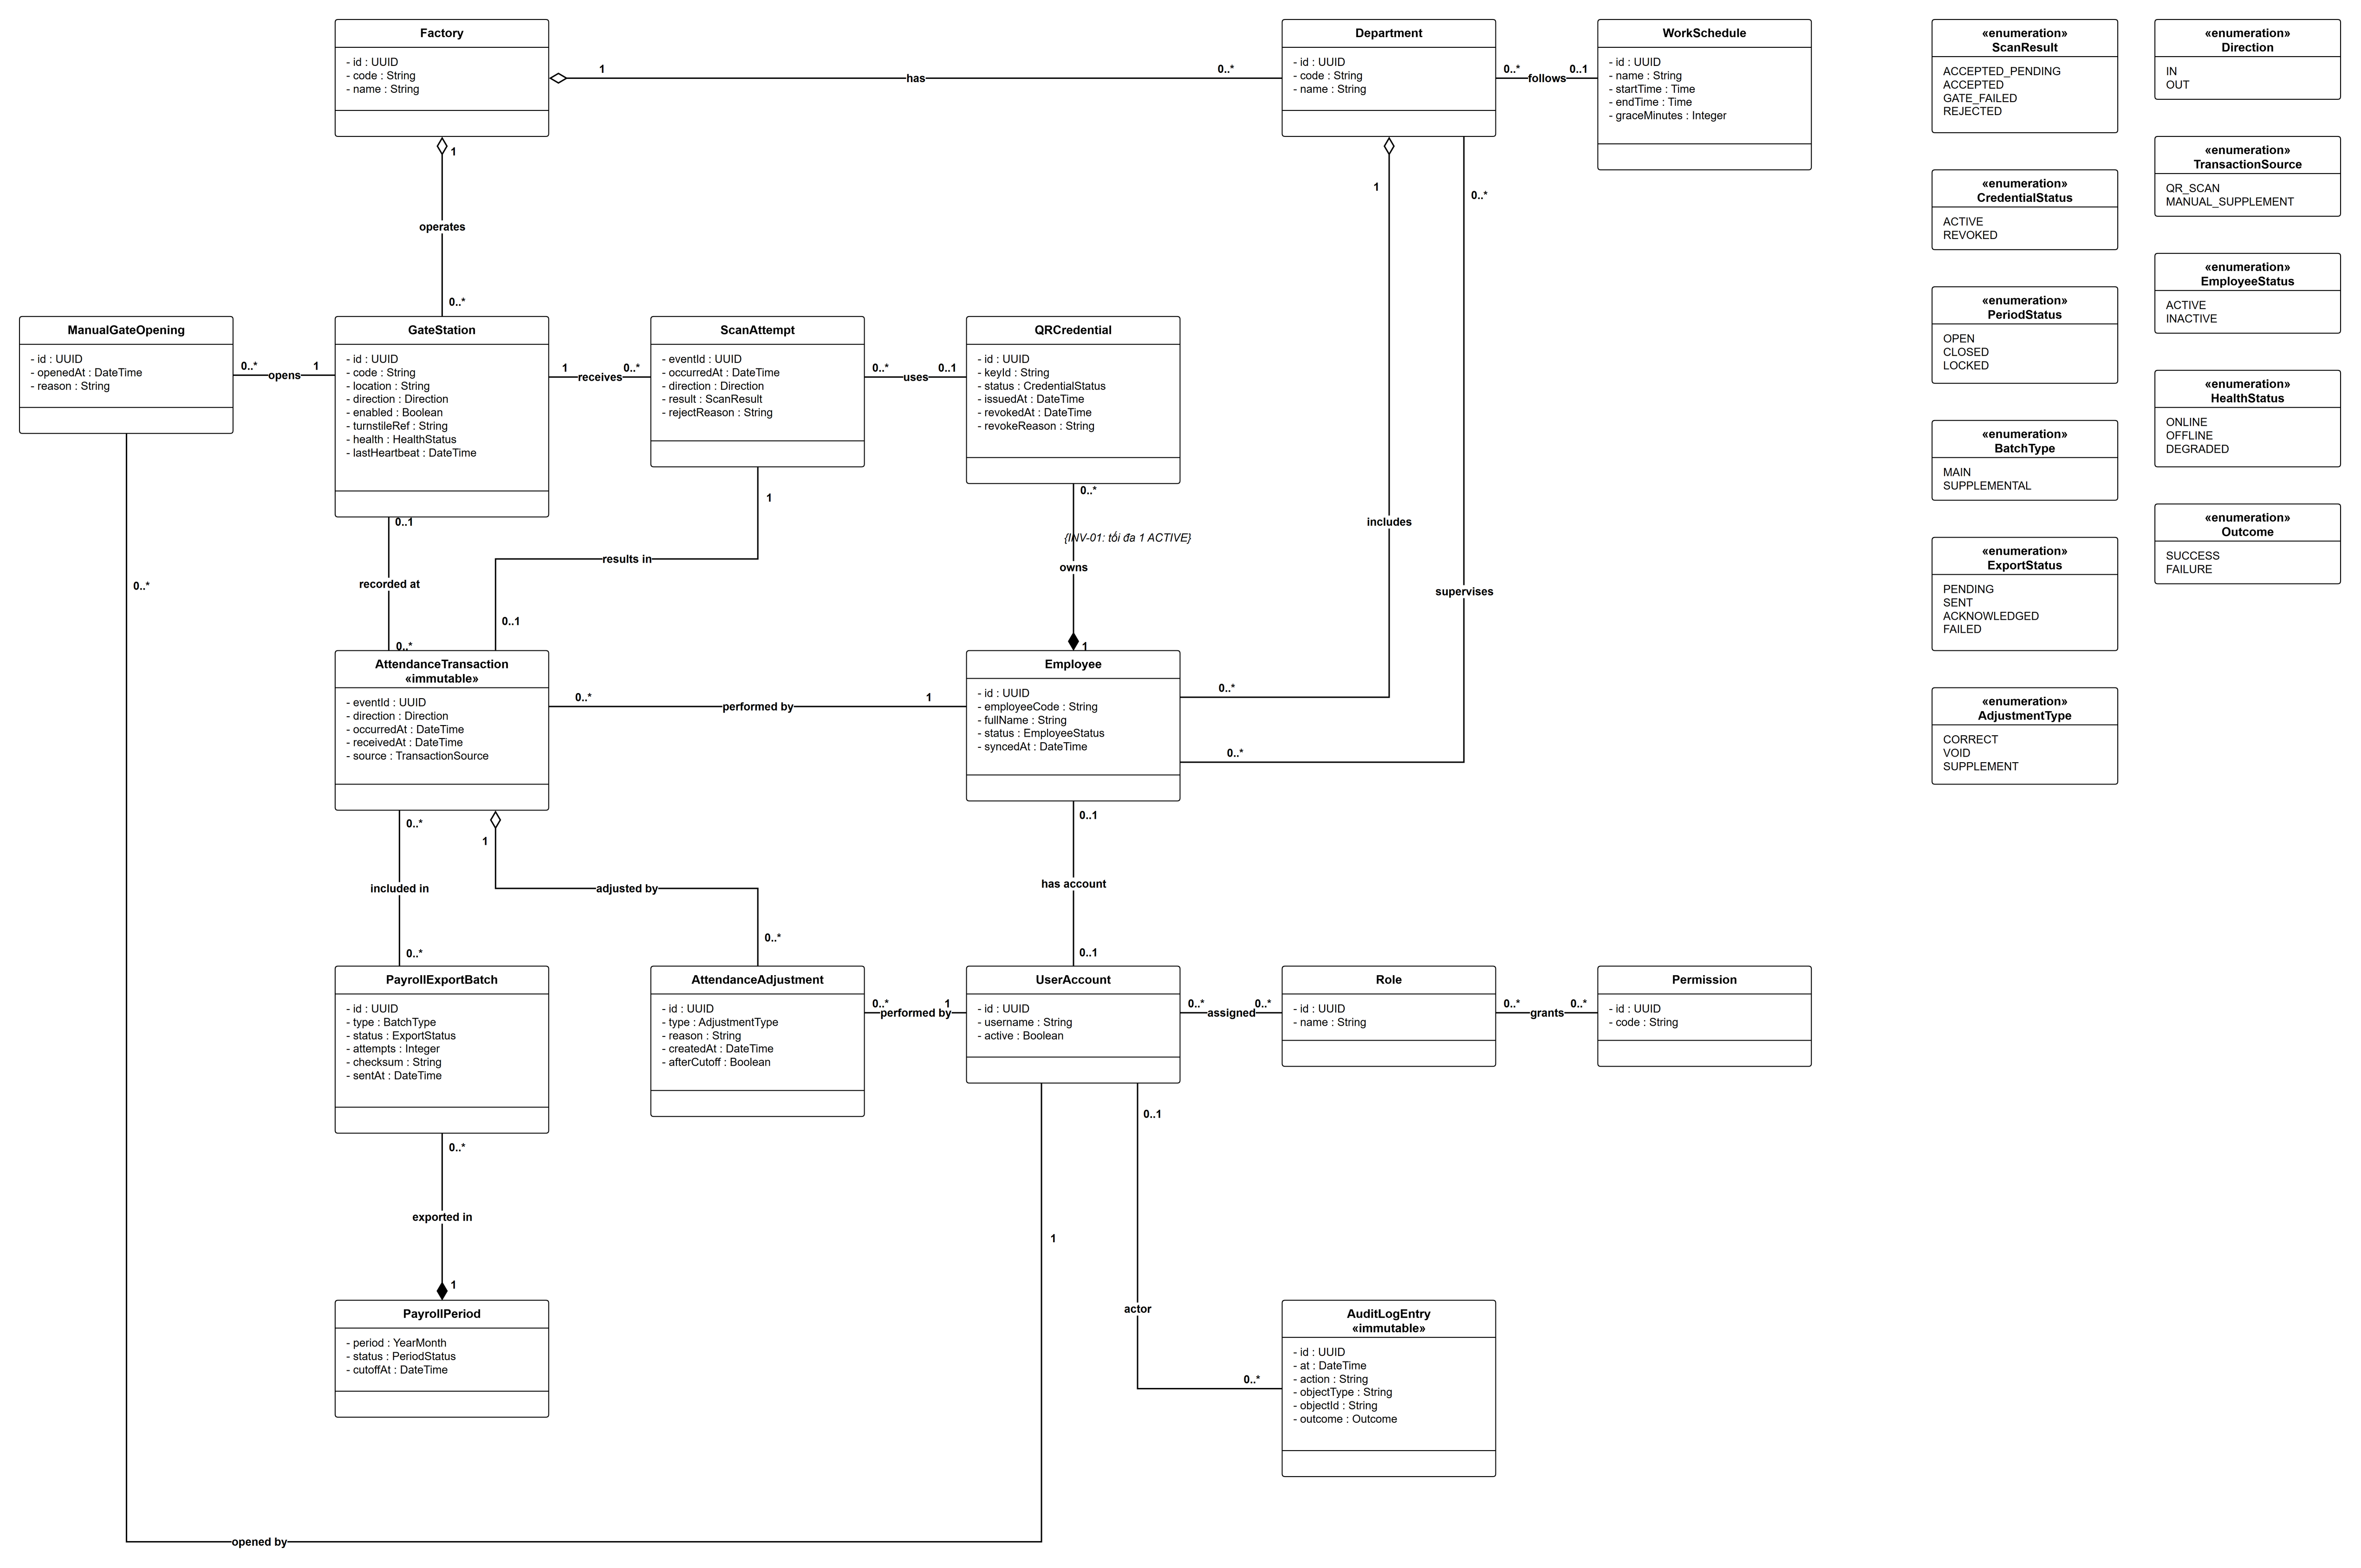
\includegraphics[width=0.92\textheight,height=0.92\textwidth,keepaspectratio]{figures/04_domain_model/class_diagram.png}}
    \caption{Lược đồ lớp mức nghiệp vụ của hệ thống chấm công và kiểm soát ra vào}
    \label{fig:sa-class-diagram}
\end{figure}
